% ============================================================
% 片段：s02b  对应原文 section2.tex 第 355--646 行；PDF 第 15--24 页
% 内容：§2 Higher-Form Symmetry（2.3 Gauging Higher-Form Symmetry；2.4 Symmetry Trifecta）
% 译者：t-s02b   审校状态：初稿
% ============================================================

% ==== 原文 PDF 第 15 页 ====

\subsection{高形式对称性的规范化}\label{sec:gauging}

一个近乎古老却又历久弥新的问题是：什么是规范化？它通常指把某个整体对称性变成规范对称性的操作。但什么是规范对称性？在某些说法中，它指的是依赖于时空的对称性，不过这会有一些限制；例如，若不放弃光滑性，如何能让一个离散对称性依赖于时空、同时又区别于整体对称性？更好的理解是对规范场的所有可能“构型”求和，从而使规范变换确定地成为冗余；关于这些表述，我们将在第~\ref{sec:three}~节中说得更为明确。本节中，除非另有说明，$p$-形式对称性群 $G^{(p)}$ 是阿贝尔的。我们把这种对称性的背景 $(p+1)$-形式规范场记为 $A^{(p+1)}$。

更准确地说，规范化有两种等价的视角：
\begin{enumerate}
    \item 对算符 $U_g(M^{d-p-1})$ 的所有可能插入求和；
    \item 把 $A^{(p+1)}$ 提升为动力学规范场，然后对 $A^{(p+1)}$ 的所有构型作积分（求和）。
\end{enumerate}
特别地，在规范化有限阿贝尔群的情形，有如下命题：
\begin{prop}
\label{prop:gauge}
    在对理论 $Z[A^{(p+1)}]$ 的有限阿贝尔对称性 $G^{(p)}$ 作规范化之后，规范化后的理论 $Z'$ 会显现一个新的对称性 $\hat{G}^{(d-p-2)}$，其中 $\hat{G}\equiv {\rm Hom}_{\rm Grp}(G,U(1))$ 是 $G$ 的 Pontryagin 对偶。规范化后的理论具有配分函数
    \be Z'[\hat{A}^{(d-p-1)}] = \sum_{[A^{(p+1)}] \in H^{(p+1)}(M^d; G^{(p)})} Z(A^{(p+1)}) \exp(2\pi i \int_{M^d} \expval{\hat{A}^{(d-p-1)},A^{(p+1)}}  ) \ , \ee
    其中 $\expval{}$ 是群层面的内积。当群 $G^{(p)}$ 连续时，$\expval{}$ 对应取值于 $\Hat{\mathfrak{g}}$ 的元素作用在取值于 $\mathfrak{g}$ 的元素上的楔积。若 $G^{(p)}$ 离散，$\expval{}$ 应解释为取值于 $\Hat{G}$ 的元素作用在取值于 $G$ 的元素上的杯积。
\end{prop}

\begin{yizhu}
(2.30) 式的求和不是对规范场构型的泛函积分，而是对\textbf{上同调类} $[A^{(p+1)}]\in H^{(p+1)}(M^d;G^{(p)})$ 求和（即只对平坦背景求和），这是“有限阿贝尔群”这一前提的直接后果，也是后文能用上同调与杯积语言的原因；对连续群，该求和须换成对联络的积分，命题的表述要另行处理。另须核对两处形式次数：规范化的对象是 $p$-形式对称性，其背景场是 $(p+1)$-形式，而规范化后出现的是 $d-p-2$ 形式的对偶对称性，其背景场为 $(d-p-1)$-形式——这正是 (2.30) 左端写 $\hat{A}^{(d-p-1)}$ 的缘由。所谓“再规范化一次回到原理论”，依赖的是 Pontryagin 对偶 ${\rm Hom}({\rm Hom}(G,U(1)),U(1))=G$，它对有限阿贝尔群成立；$\expval{}$ 在连续/离散两种情形分别取楔积与杯积，勿混用。
\end{yizhu}

\begin{proof}
    在开始证明之前，先体会一下该定理的直观。按朴素的看法，对具有 0-形式对称性的理论作规范化，应当相当于把希尔伯特空间投影到物理的希尔伯特空间，但并不尽然。该投影是非可逆的，而为了保留%
% ==== 原文 PDF 第 16 页 ====
表示的信息，我们可以插入一条威尔逊线（回忆一下，威尔逊线由所选表示标记）。

    因此这里我们也照此办理。耦合项
    \[\exp(2\pi i \int_{M^d} \expval{\hat{A}^{(d-p-1)},A^{(p+1)}}  ) \ , \]
    可以看作耦合了一个离散通量。依照此前的方法，理论 $Z$ 中的对称性算符应由该离散通量构造（它是威尔逊线的更高维版本）\cite{Schafer-Nameki:2023jdn}
    \be D(M^{d-p-1} ) = \exp(i\int_{M^{d-p-1}} \hat{A}^{(d-p-1)}) \ . \ee
    但有什么地方不对：$\hat{A}^{(d-p-1)}$ 取值于 $\Hat{G}$ 而非 $G$！这里的正确理解是：\textbf{融合规则仍是 $G$ 的乘法}，这通过把算符正确写成
    \be D(\rho, M^{d-p-1}) = \rho\Big( \exp(i\int_{M^{d-p-1}} \hat{A}^{(d-p-1)})\Big) \ , \ \rho\in {\rm Rep}(\Hat{G}) = G \ .  \ee
    来实现。于是对称性算符的融合规则为
    \be D(\rho_1 ,M ) \otimes D(\rho_2,M) = D(\rho_1\otimes \rho_2 ,M)   \ee
    它正确地以 $G$ 的乘法作为融合规则。\footnote{感谢 Ruizhi Liu 对这部分的有益讨论。}

    类似地，对于规范化后的理论 $Z'$，对称性算符构造为
    \be D'(\rho', M^{p+1}) = \rho'\Big( \exp(i\int_{M^{p+1}} A^{(p+1)}) \Big)\ , \ \rho'\in {\rm Rep}(G) = \Hat{G} \ . \ee
    既然对称性算符已构造出来，我们就可以合理地说 $Z'$ 理论具有 $\Hat{G}^{(d-p-2)}$ 对称性。
\end{proof}

\begin{yizhu}
证明中“但有什么地方不对”这一步是全段的枢纽，作者只用一句话带过，其实质是：$\hat{A}^{(d-p-1)}$ 是 $\Hat{G}$ 值的，故 $\exp(i\oint\hat{A})$ 本身并不按 $G$ 的元素标记，直接用它会得到错误的融合规则。修补办法是把 $\Hat{G}$ 的表示（特征标）$\rho\in{\rm Rep}(\Hat{G})$ 复合上去；由 Pontryagin 对偶 ${\rm Rep}(\Hat{G})=G$，$\rho_1\otimes\rho_2$ 恰好对应 $G$ 中的乘法 $g_1g_2$，于是融合规则 (2.33) 自动成立。反过来，对偶理论 $Z'$ 的算符用 $\rho'\in{\rm Rep}(G)=\Hat{G}$ 构造，两套算符的形式完全对称——这正是“再规范化一次回到原理论”的来源。此处不必也不应把 $\rho$ 理解成矩阵的迹：它只承担“把 $\Hat{G}$ 值翻译成 $G$ 值”的角色。
\end{yizhu}

作为推论，我们实际上可以对 $\hat{G}^{(d-p-2)}$ 再作一次规范化，从而回到原来的理论。这只是一个简单的练习：只需注意到 ${\rm Hom}( {\rm Hom}(G,\U(1)) , U(1) ) = G$ 以及 $d-(d-p-2)-2 = p$。

\subsubsection{$p$-形式对称性的 't Hooft 反常}

然而，在某些情形下规范化无法完美实施，可能存在障碍，我们称之为 't Hooft 反常。它是规范变换导致理论配分函数发生改变的现象。
% ==== 原文 PDF 第 17 页 ====
也就是说，若取 $\delta_\lambda A$ 为背景规范场的一般变换\footnote{对无穷小规范变换，它称为\textbf{局域反常}；对大规范变换，它称为\textbf{整体反常}。}，
\be Z(A + \delta_\lambda A) = \exp(2\pi i \int_{M^d} I_d)\cdot  Z(A) \  \ee
其中 $I_d$ 是由规范场构成的 $d$-形式。当然，只有当这样的相位因子 $2\pi i \int_{M^d} I_d$ 无法被 $d$ 维作用量中规范不变的局域抵消项消去时，我们才说该系统具有 't Hooft 反常。

处理该问题的一个标准做法是通过下降公式（descent formula）。其想法是找一个规范不变的客体来描述反常。下降公式为
\be
\ba
\dd I_d = \delta_\lambda I_{d+1} \ , \ \dd I_{d+1}  = I_{d+2} \cr
Z(A + \delta_\lambda A) = \exp(2\pi i \int_{M^{d+1}} \delta_\lambda I_{d+1})\cdot  Z(A)
\ea
\ee
其中 $\ptl M^{d+1} = M^d $。$I_{d+1}$ 是 $(d+1)$-形式 't Hooft 反常多项式，$I_{d+1} $ 是规范不变的 $(d+2)$-形式。

\begin{yizhu}[原文疑误]
(2.36) 之后一句原文（源码第 410 行，PDF 第 17 页同）为“$I_{d+1}$ 是 $(d+1)$-形式 't Hooft 反常多项式，$I_{d+1}$ 是规范不变的 $(d+2)$-形式”：第二个 $I_{d+1}$ 显然应为 $I_{d+2}$（否则与 $(d+2)$-形式自相矛盾，也与上一行 $\dd I_{d+1}=I_{d+2}$ 冲突）。此处照原文保留符号，读者应按 $I_{d+2}$ 理解。顺带说明这条下降链的标准读法：$I_{d+2}$ 是闭的不变多项式，$I_{d+1}$ 是其陈–西蒙斯型“势”，$\delta_\lambda I_{d+1}=\dd I_d$ 给出反常的局域形式；作者把两条关系并排写成一个公式，读取时不要误以为 $\delta_\lambda I_d$ 也参与同一等式。
\end{yizhu}

这给出“反常流入”（anomaly inflow）机制的线索：$d$ 维的 QFT 可以与 $(d+1)$ 维的 QFT 耦合。一个一般的构造是：如上定义、带有 't Hooft 反常的 $M^d$ 上的 QFT，可以与 $M^{d+1}$ 上取 $\mathcal{L} = -2\pi I_{d+1}$ 的 TQFT 耦合。整个理论是良定义的、无反常的理论。这一概念与凝聚态物理中对称保护拓扑（SPT）相的概念直接相关~\cite{gu2009tensor,chen2012symmetry,chen2013symmetry,chen2011two,levin2012braiding,PhysRevB.89.035147,chenjie2014,chenjie2015,senthil2015symmetry}；在那里，对称性正是我们正在规范化的那个整体对称性。SPT 相是非相互作用的拓扑绝缘体与超导体的相互作用推广~\cite{TI01,TI02,TI1,TI2,TI3,TI4,TI5}，它们具有受对称性保护的稳健边界态与拓扑性质。

下面给出高形式对称性规范化与 't Hooft 反常的一些例子。

\subsubsection{例：带背景场的麦克斯韦理论}

现在考虑一个 4 维 $U(1)$ 麦克斯韦理论，它具有 $U(1)_E$、$U(1)_M$ 1-形式对称性，并耦合背景规范场 $B_E$、$B_M$，则耦合后的作用量成为
\be 
\label{Maxwell-gauged}
S = \frac{1}{2e^2} \int (F-B_E)\wedge * (F-B_E) + \frac{1}{2\pi} \int (F-B_E)\wedge B_M\,,  
\ee
规范变换为
\be  A\mapsto A + \lambda_E  \ , \ B_E \mapsto B_E + \dd \lambda_E \ , \ B_M \mapsto B_M + \dd \lambda_M \ee
因此 $(F-B_E)$ 是规范不变的；另需注意，这里允许 $\lambda_E$ 与 $\lambda_M$ 非平坦。

% ==== 原文 PDF 第 18 页 ====
在这种规范变换下，
\be
\delta S = -\frac{1}{2\pi} \int_{M^4} B_E\wedge \dd\lambda_M\,.
\ee
因此作用量不是规范不变的，该理论具有混合 't Hooft 反常；这意味着我们不能同时规范化 $U(1)_E \ $与$ \ U(1)_M$。提升到 5 维后，'t Hooft 多项式为
\be I_5=-\frac{1}{(2\pi)^2} \dd B_E \wedge B_M \ . \ee
注意，耦合后的作用量~(\ref{Maxwell-gauged}) 的选取使得非规范不变项的数目最少。

若取组合系统
\be S_{\rm 5d-4d} = \frac{1}{2e^2} \int_{M^4} (F-B_E)\wedge * (F-B_E) + \frac{1}{2\pi} \int_{M^4} (F-B_E)\wedge B_M+\frac{1}{2\pi}\int_{M^5}dB_E\wedge B_M\,, \ee
则整个系统是规范不变的。

\subsubsection{例：3 维 $U(1)$ 陈–西蒙斯理论}

3 维 $U(1)$ 陈–西蒙斯理论的基本设定为
\be\ba S &= \frac{\kappa}{4\pi} \int_{M^3} A\wedge \dd A  \ \ \kappa\in\bbZ \cr  {\rm e. o. m. :} \ \ \dd A &= 0 \ea \ee
这里 $\kappa\in \bbZ$ 是量子化的陈–西蒙斯能级（level）。

该系统具有 $\bbZ_\kappa^{(1)}$ 1-形式对称性。在 3 维中，1-形式对称性具有 $3-1-1=1$ 维的拓扑线算符（或缺陷），而其所作用的对象也是 1 维的线。该理论中自然地只有一个规范不变的线算符：威尔逊圈\footnote{这里没有前文 4 维麦克斯韦理论中提到的 't Hooft 线，因为电磁对偶的要求体现在拉氏量中。换言之，麦克斯韦理论的磁对称性被陈–西蒙斯项破坏。}。下文记 $g_n\equiv \exp(2\pi i n/\kappa)$。线算符为
\be  U_{g_n} (\gamma)= \exp(i n \oint_\gamma A) \ , \ \gamma:[0,1]\to M, \gamma(0) = \gamma(1) \ .   \ee
因此，作用在线上的效果为
\be U_{g_m} (\gamma_1) U_{g_n} (\gamma_2) = \exp(\frac{2\pi i m n}{\kappa} \expval{\gamma_1, \gamma_2}) U_{g_n} (\gamma_2) \ .  \ee
对此的另一种视角是：拓扑算符 $ U_{g_n} (\gamma)$ 把 $A$ 平移一个平坦联络，$A\mapsto A + \frac{n}{\kappa} \epsilon$。

% ==== 原文 PDF 第 19 页 ====
若规范化 $\bbZ_\kappa^{(1)}$ 对称性，我们会遇到 $3-1-2 = 0$-形式的 $\hat{\bbZ}_\kappa = \bbZ_\kappa $ 对称性。规范化过程通过对 $U_{g_n}$ 的所有可能插入求和来实现。规范化之后，理论变为
\be \ba
A' &= \kappa A\cr
S &= \frac{1}{4\pi \kappa} \int_{M^3} A' \wedge \dd A' \quad, \  \kappa\in\bbZ  \ .
\ea\ee
现在 $A'$ 是恰当量子化的规范场。

然而，新理论在 $A'$ 的大规范变换下不再规范不变。为不熟悉 CS 理论的读者，我们概述一下陈–西蒙斯能级量子化背后的论证（另见 \cite{TongGauge} 第 8.4 节）。考虑陈–西蒙斯作用量
\be
S=\frac{\kappa}{4\pi}\int_{M^3} A\wedge \dd A
\ee
它定义在 $M^3=S^1\times S^2$ 上。我们把欧氏时间方向 $S^1$ 取为 $x^0\sim x^0+2\pi R$ 方向，把 $S^2$ 取为 $x^1$、$x^2$ 方向。引入磁通量 $\int_{S^2}F=2\pi$。现在考虑大规范变换 $A_\mu\rightarrow A_\mu+\ptl_\mu \lambda$，其中 $\lambda=x^0/R$ 绕 $S^1$ 缠绕。于是在该规范变换下，有 $A_0\rightarrow A_0+1/R$，而规范场 $A_0$ 现在具有周期 $1/R$。为讨论 CS 作用量的规范变换，我们考虑 $A_0$ 为常数的构型，并化简得
\be
\ba
S&=\frac{\kappa}{4\pi}\int_{S^1\times S^2} A\wedge \dd A\cr
&=\frac{\kappa}{4\pi}\int_{S^1\times S^2}A_0 F_{12}+A_1 F_{20}+A_2 F_{01}\cr
&=\frac{\kappa}{2\pi}\int_{S^1\times S^2}A_0 F_{12}\,.
\ea
\ee
作大规范变换后
\be
\ba
\delta S&=\frac{\kappa}{2\pi}\int_{S^1\times S^2}\frac{1}{R} F_{12}\cr
&=2\pi\kappa\,.
\ea
\ee
因此，为保持 $e^{iS}$ 不变，要求 $\kappa\in\mb{Z}$。

现在我们要计算规范化 $\mb{Z}_\kappa$ 1-形式对称性之后的 't Hooft 反常多项式。我们要求 $M^3$ 是自旋流形，且是某个 4 维自旋流形 $M^4$ 的边界。可把作用量改写为
\be S = \frac{\kappa}{4\pi} \int_{M^3} A\wedge \dd A =  \frac{\kappa}{4\pi} \int_{M^4} F\wedge F = 2\pi \kappa \int_{M^4} \frac{c_1^2}{2}  \ee
% ==== 原文 PDF 第 20 页 ====
其中 $c_1 = \frac{F}{2\pi}$ 是以 $A$ 为联络的主丛的第一陈类。接着把系统与取值于 $\bbZ_\kappa$ 的背景规范场 $B\in H^2 (M^3;\bbZ_\kappa)$ 耦合，把作用量变为
\be S \mapsto S =  \frac{\kappa}{4\pi} \int_{M^4} (F -\frac{2\pi}{\kappa} B)\wedge (F -\frac{2\pi}{\kappa} B)  \ ,\ee
若允许非平坦的规范变换 $A\mapsto A +\epsilon/\kappa$，它便不是规范不变的，因为 $B$ 取值于 $\bbZ_\kappa$，无法承受小规范变换。因此反常多项式项为
\be I_4 = \frac{1}{2\kappa} \int_{M^4} B\cup B  \ .  \ee
若 $I_4\notin \bbZ$，我们就会遇到 't Hooft 反常。此前要求 $M^4$ 为自旋流形这一条件给出
\be \int_{M^4} B\cup B  \in 2\bbZ \Rightarrow I_4\in \bbZ/\kappa \ , \ee
故当 $\kappa > 1 $ 时理论有反常。

\begin{yizhu}
(2.52) 中的 $\bbZ/\kappa$ 不是在说商群 $\bbZ/\kappa\bbZ$，而应读作 $\frac{1}{\kappa}\bbZ$，即 $I_4$ 取值为 $\kappa$ 次单位根的对数：自旋条件保证 $\int B\cup B\in 2\bbZ$，于是 $I_4=\frac{1}{2\kappa}\int B\cup B\in\frac{1}{\kappa}\bbZ$，$e^{2\pi iI_4}$ 才是 $\kappa$ 次单位根。这也解释了为何 $\kappa=1$ 时无反常（$I_4\in\bbZ$，相位为 1）、而 $\kappa>1$ 时有反常。另请核对 (2.50) 处的平移约定 $A\mapsto A+\epsilon/\kappa$ 与 (2.45) 的 $A'=\kappa A$ 是否自洽：正因 $A'$ 是“恰当量子化”的场，其大规范变换才在 CS 项上产生非平凡相位，这正是本段要说明的要点。
\end{yizhu}

\subsection{对称性三要素}\label{sec:three}

至此我们已大致理解了用拓扑缺陷语言表述的高形式对称性，并在一些情形中提到它也可以看作对平坦联络的平移。有了前面的例子，我们现在可以向前推进，对高形式对称性作更透彻的理解。我们的断言是：高形式对称性可以从三种可互换的视角来把握：\textbf{拓扑缺陷网络}（TDN）、\textbf{平坦联络}与\textbf{分类空间}。

我们先在 0-形式对称性范围内定义这些视角，然后再把它们推广到高形式对称性。

\begin{enumerate}
    \item \textbf{拓扑缺陷网络}。对于已经熟悉拓扑算符的读者，可径行跳到下一项关于平坦联络的内容。下面我们以格点视角为重点深入这一主题。

    考虑贯穿 $d$ 维空间的一系列格点，每个格点都关联一个希尔伯特空间 $\CH_i$，例如一个量子比特对应 $\mathbb C^2$。系统随时间的演化一直进行，直到遇到一个打断其连续性的拓扑缺陷。图~\ref{Fig:lattice-TDN} 给出了这一概念在 $1+1$ 维情形下的直观表示。

% ==== 原文 PDF 第 21 页 ====
\begin{figure}[htbp]
  \centering
  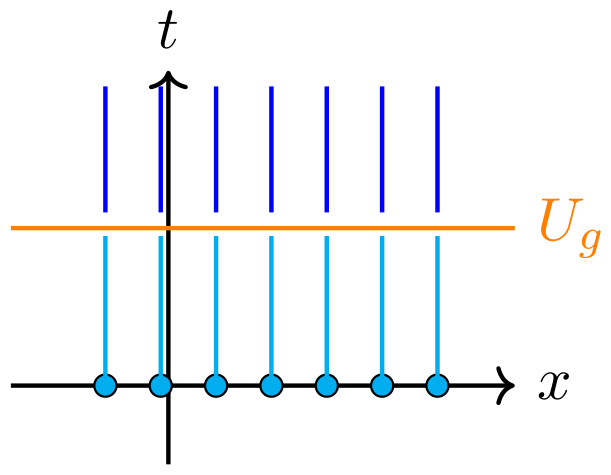
\includegraphics[width=0.24\linewidth]{figures/figure-5.png}
  \caption{带拓扑缺陷的一维格点。（原文 Figure~5，PDF 第 21 页）}
  \label{Fig:lattice-TDN}
\end{figure}

    拓扑缺陷算符必须遵从群的表示，这可以写成
    \be U_{g} U_{h} = U_{gh}. \ee
    该运算可以理解为拓扑缺陷 $U_g$ 与 $U_h$ 融合为 $U_{gh}$，如下式所示：
    \be
        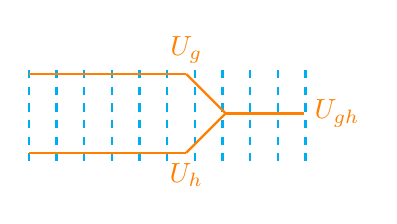
\begin{tikzpicture}
        \draw[color = cyan, thick,dashed] (-1,0.05)--(-1,-1.2)
        [shift = {(10pt,0)}] (-1,0.05)--(-1,-1.2)
        [shift = {(10pt,0)}] (-1,0.05)--(-1,-1.2)
        [shift = {(10pt,0)}] (-1,0.05)--(-1,-1.2)
        [shift = {(10pt,0)}] (-1,0.05)--(-1,-1.2)
        [shift = {(10pt,0)}] (-1,0.05)--(-1,-1.2)
        [shift = {(10pt,0)}] (-1,0.05)--(-1,-1.2)
        [shift = {(10pt,0)}] (-1,0.05)--(-1,-1.2)
        [shift = {(10pt,0)}] (-1,0.05)--(-1,-1.2)
        [shift = {(10pt,0)}] (-1,0.05)--(-1,-1.2)
        [shift = {(10pt,0)}] (-1,0.05)--(-1,-1.2);

        \draw[orange, thick] (-1,0)--(1,0) node[anchor = south]{$U_g$};
        \draw[orange, thick] (-1,-1)--(1,-1) node[anchor = north]{$U_h$};
        \draw[orange, thick] (1,0)--(1.5,-0.5);
        \draw[orange, thick] (1.5,-0.5)--(2.5,-0.5) node[anchor = west]{$U_{gh}$};
        \draw[orange, thick] (1,-1)--(1.5,-0.5);


        \end{tikzpicture}
    \ee
    式中蓝色虚线表示各格点上状态的时间演化。需要注意，由缺陷实现的群作用应当是有向的；反方向对应于逆算符 $U_{g^{-1}}$。例如，依次作用缺陷算符 $U_g$、$U_{g^{-1}}$、$U_g$，其结果应与单独作用一次 $U_g$ 相同：
    \be
        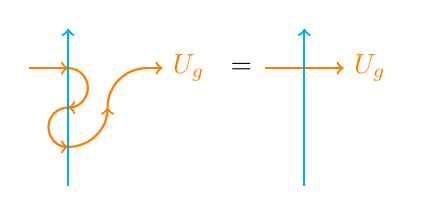
\begin{tikzpicture}
        \draw[orange , thick , ->] (-1,1)--(-0.5,1) ; 
        \draw[orange , thick,->] (0.5,1)--(0.7,1) node[anchor = west]{$U_g$}; 
        \draw[orange , thick,->] (2,1)--(3,1) node[anchor = west]{$U_g$}; 
        \draw[orange,thick,->] (-0.5,1) arc (90:-90:0.25);
        \draw[orange,thick,->] (-0.5,0.5) arc (90:270:0.25);
        \draw[orange,thick,->] (-0.5,0) arc (-90:0:0.5);
        \draw[orange,thick] (0,0.5) arc (180:90:0.5);
        \draw[cyan,thick,->] (-0.5,-0.5) -- (-0.5,1.5);
        \draw[cyan,thick,->] (2.5,-0.5) -- (2.5,1.5);

        \node[] at (1.7,1) {$=$};
        \end{tikzpicture}
    \ee

    此外，$U_{g^{-1}}$ 与 $U_g$ 的逆关系可以表示为：
    \be\label{Prop:bubble}
        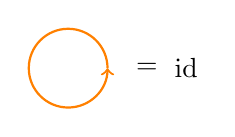
\begin{tikzpicture}
        \draw[thick, orange ,->] (-0.5,0) arc (0:360:0.5);
        \node[] at (0,0) {$=$};%{$\propto$};
        \node[] at (0.5,0) {id};
        \end{tikzpicture}
    \ee
    这样的“气泡”总可以加入 TDN 中，而实际上不改变尊重该对称性的系统。

    \item \label{para:flatconn}\textbf{平坦联络}。在格点规范理论、或等价地在 Čech 上同调的语境中，我们用 $i$、$j$、$k$ 等指标给格点贴标签。1-形式规范联络（记为 $A$）负责把群元素赋给连接格点的连线（link）。也就是说，若格点 $i$ 与格点 $j$ 之间有一条连线，则 $A_{ij} \in G$，其中 $G$ 是我们所研究的群。然而这一赋值并非任意，它必须服从特定条件，例如
    \be A_{ij}\cdot A_{jk} \cdot A_{ki} = {\rm id} = A_{ij} \cdot A_{ji} \ . \label{Eq:Flatcondition}\ee
% ==== 原文 PDF 第 22 页 ====
    这一条件刻画了所谓平坦联络。事实上，在连续极限下，式~(\ref{Eq:Flatcondition}) 可以解释为线积分
    \be  \oint A = 0. \ee
    此情形下的规范变换为
    \be\label{gaugetransf1} A_{ij} \mapsto A_{ij}'=g_i^{-1} A_{ij} g_j,  \ee
    从而
    \be \int_{i\to j} A = A_{ii_1}\cdot A_{i_1 i_2}\dots A_{i_n j} \mapsto g_i^{-1} \cdot (\int_{i\to j} A) \cdot g_j. \ee
    若取闭合回路作积分，我们看到威尔逊圈是规范不变的，正如所预期。

    \item \textbf{分类空间}。这是一个更为抽象的概念；本节旨在提供直观理解，而非严格证明。主要想法是构造一个空间 $BG$，使得任何主丛 $P\to M$ 都可以通过一个映射 $\phi : M\to BG$ 拉回得到，如图~\ref{Fig:ClassSpace} 所示。在此语境中，$EG\to BG$ 表示“万有 $G$-丛”，它可被拉回而给出任意 $G$-丛。这看起来或许复杂，但若回想我们此前对平坦联络的理解，就能看出真正重要的是把群元素赋给连接各格点的连线的信息；格点本身的细节对我们的目的而言变得不那么重要。更详细的描述请参见例~\ref{Eg:GT}。指定一个规范场构型本质上等价于定义各路径的和乐，而这又对应于从时空到分类空间 $BG$ 的映射。
    \begin{figure}[htbp]
        \centering
            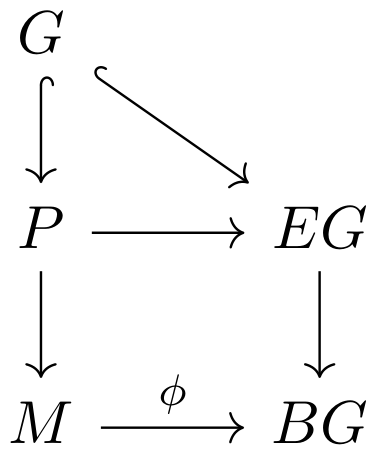
\includegraphics[width=0.15\linewidth]{figures/figure-6.png}
        \caption{分类空间与万有丛。（原文 Figure~6，PDF 第 22 页）}
        \label{Fig:ClassSpace}
    \end{figure}

\begin{definition}
群 $G$ 的分类空间（记作 $BG$）是一个拓扑空间，它具有性质 $\pi_1(BG) \cong G$，而对所有不等于 1 的 $n$ 都有 $\pi_n(BG) = 0$。
\end{definition}

% ==== 原文 PDF 第 23 页 ====
映射 $\phi: M\to BG$ 把时空流形 $M$ 中的点映到分类空间 $BG$ 中的那个单点，并把 $M$ 中的路径映到群元素，如前所述。必须认识到，同伦等价的映射 $\phi$ 给出时空流形 $M$ 上等价的 $G$-丛。从规范场联络的角度看，这种等价对应于式~(\ref{gaugetransf1}) 中规范等价的规范场构型 $A$ 与 $A'$。这样，数学中同伦的概念就翻译成了物理中规范变换的概念。

\end{enumerate}

把前述三种视角从 0-形式对称性推广到高形式对称性是一个直接的过程。下面给出概览：

\begin{enumerate}
    \item \textbf{拓扑缺陷网络}（几何直观）。在这一视角下，拓扑缺陷是嵌入 $d$ 维时空中的 $(d-p-1)$ 维对象。这些对象能够沿更低维的流形彼此结合或相互作用。缺陷网络为理解高 $p$-形式对称性在给定物理系统中如何作用提供了一份独特而精确的指南；它勾勒出该对称性作用于系统的规则与模式。这一做法给我们以几何直观，因为所有算符都关联于时空流形内的子流形。

    \item \textbf{平坦联络}（物理计算）。在此语境中，联络取 $(p+1)$-形式，它建立群元素与时空流形中 $(p+1)$-单纯形之间的赋值。例如，1-形式对称性对应 2-形式规范场。在格点框架中，这些规范场把群元素（对阿贝尔群 $G$ 记为 $g_{ijk}$）赋给时空流形三角剖分中的三角形，后者记为 $\langle ijk\rangle$。这些联络同样受平坦联络条件的约束，这意味着与一个四面体边界上全部四个三角形相联系的群元素之和等于 $G$ 中的平凡元素。这一做法的优点是：我们可以容易地用规范场写出作用量与规范变换规则，因而很适合物理计算。
    
    \item \textbf{分类空间}（拓扑分类）。我们现在有分类映射 $\phi: M^d\to B^{p+1}G$，其中 $B^{p+1}G=K(G,p+1)$ 是 Eilenberg–MacLane 空间，其定义为 $\pi_{p+1}(B^{p+1}G) \cong G$，而所有其他同伦群平凡。
% ==== 原文 PDF 第 24 页 ====
从时空流形 $M^d$ 到 Eilenberg–MacLane 空间的映射，等价于把 $G$ 中的群元素赋给时空流形三角剖分的 $(p+1)$ 维单纯形。这些赋值自动满足平坦联络条件。这一做法把物理问题转化为同伦问题，因而适用于分类，例如理解高形式对称性中的反常。
    
    \end{enumerate}
